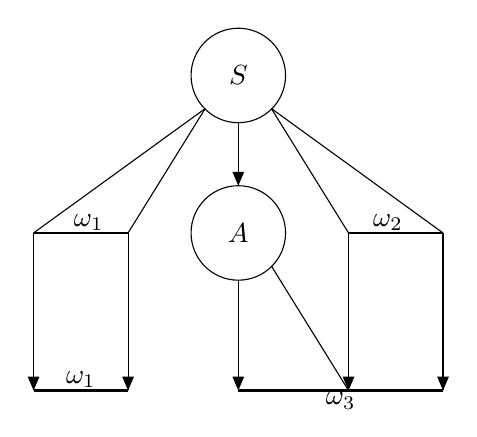
\begin{tikzpicture}[scale=0.2]
\tikzstyle{every node}+=[inner sep=0pt]
\draw [black] (0,0) circle (3);
\draw (0,0) node {$S$};

\draw [black] (-2.1, -2.1) -- (-7,-10);
\draw [black] (-2.1, -2.1) -- (-13,-10);
\draw [black, thick] (-7,-10) -- (-13, -10);
\draw (-9.5, -9.875) node [above] {$\omega_1$};

\draw [black] (0, -3) -- (0, -7);
\fill [black] (0, -7) -- (-.375, -6.125) -- (+.375, -6.125);
\draw [black] (0, -10) circle (3);
\draw (0, -10) node {$A$};

\draw [black] (+2.1, -2.1) -- (7,-10);
\draw [black] (+2.1, -2.1) -- (13,-10);
\draw [black, thick] (7,-10) -- (13, -10);
\draw (+9.5, -9.875) node [above] {$\omega_2$};

\draw [black] (-7, -10) -- (-7,-20);
\fill [black] (-7, -20) -- (-7.375, -19.125) -- (-6.625, -19.125);
\draw [black] (-13, -10) -- (-13,-20);
\fill [black] (-13, -20) -- (-13.375, -19.125) -- (-12.625, -19.125);
\draw [black, thick] (-7,-20) -- (-13, -20);
\draw (-10, -19.875) node [above] {$\omega_1$};

\draw [black] (0, -13) -- (0,-20);
\fill [black] (0, -20) -- (-.375, -19.125) -- (+.375, -19.125);
\draw [black] (+2.1, -12.1) -- (7,-20);
\draw [black] (+7, -10) -- (+7,-20);
\fill [black] (+7, -20) -- (+7.375, -19.125) -- (+6.625, -19.125);
\draw [black] (+13, -10) -- (+13,-20);
\fill [black] (+13, -20) -- (+13.375, -19.125) -- (+12.625, -19.125);
\draw [black, thick] (0,-20) -- (+13, -20);
\draw (+6.5, -20.125) node [below] {$\omega_3$};
\end{tikzpicture}
